% Seccion: Partes interesadas
% Autor de la seccion: Jonathan Javier Rivera Suarez
% Version preliminar: la clasificacion se valida con la entrevista (preguntas 07 y 16).

\section{Partes interesadas}
\label{sec:partes-interesadas}

Una parte interesada es toda persona, grupo u organización que influye en el sistema o resulta afectada por él, y cuyos intereses deben considerarse al definir los requisitos \cite{iso29148}. Para el SGMC se identificaron diez roles a partir del recorrido de un microcrédito: solicitud, evaluación, aprobación, desembolso, cobro y control. Los roles se registran sin nombres personales.

La Tabla~\ref{tab:partes-interesadas} resume, para cada rol, su interés en el sistema, su nivel de influencia, la disponibilidad estimada para participar en la elicitación y la estrategia de participación propuesta. La disponibilidad es una estimación inicial y se confirmará con la organización durante la primera entrevista.

\begin{table}[htbp]
\centering
\caption{Partes interesadas del SGMC (versión preliminar).}
\label{tab:partes-interesadas}
\small
\begin{tabularx}{\textwidth}{@{}>{\raggedright\arraybackslash}p{2.6cm}>{\raggedright\arraybackslash}X>{\raggedright\arraybackslash}p{1.2cm}>{\raggedright\arraybackslash}p{1.5cm}>{\raggedright\arraybackslash}p{2.4cm}@{}}
\toprule
\textbf{Rol} & \textbf{Interés principal} & \textbf{Influ\-encia} & \textbf{Disponi\-bilidad} & \textbf{Estrategia} \\
\midrule
Comité de crédito & Decidir con información completa y con constancia de cada resolución. & Alta & Baja & Gestionar de cerca \\
Dirección Financiera / Tesorería & Controlar desembolsos, cobros y el estado de la cartera. & Alta & Media & Gestionar de cerca \\
Analista de crédito & Reducir el tiempo de revisión de expedientes y evitar datos incompletos. & Alta & Alta & Gestionar de cerca \\
Rectorado & Que el servicio cumpla la normativa y no genere riesgo institucional. & Alta & Baja & Mantener satisfecho \\
Auditoría interna & Disponer de trazabilidad de las operaciones y de reportes verificables. & Alta & Baja & Mantener satisfecho \\
Unidad de TIC & Que el sistema se integre a la infraestructura y sea mantenible. & Alta & Media & Mantener satisfecho \\
Solicitante / beneficiario & Solicitar con pocos trámites y conocer el estado y las cuotas de su crédito. & Baja & Media & Mantener informado \\
Gestor de cobranza & Identificar a tiempo las cuotas vencidas y registrar las gestiones. & Baja & Alta & Mantener informado \\
Garante & Conocer la obligación que asume y su vigencia. & Baja & Baja & Monitorear \\
Asesoría jurídica & Que contratos y garantías tengan validez legal. & Baja & Baja & Monitorear \\
\bottomrule
\end{tabularx}
\end{table}

\subsection{Matriz poder--interés}

La Figura~\ref{fig:matriz} ubica los roles según su poder sobre las decisiones del proyecto y su interés en el sistema. Su fuente editable es el archivo \texttt{matriz\_poder\_interes.puml} de la carpeta \texttt{modelos}.

\begin{figure}[htbp]
\centering
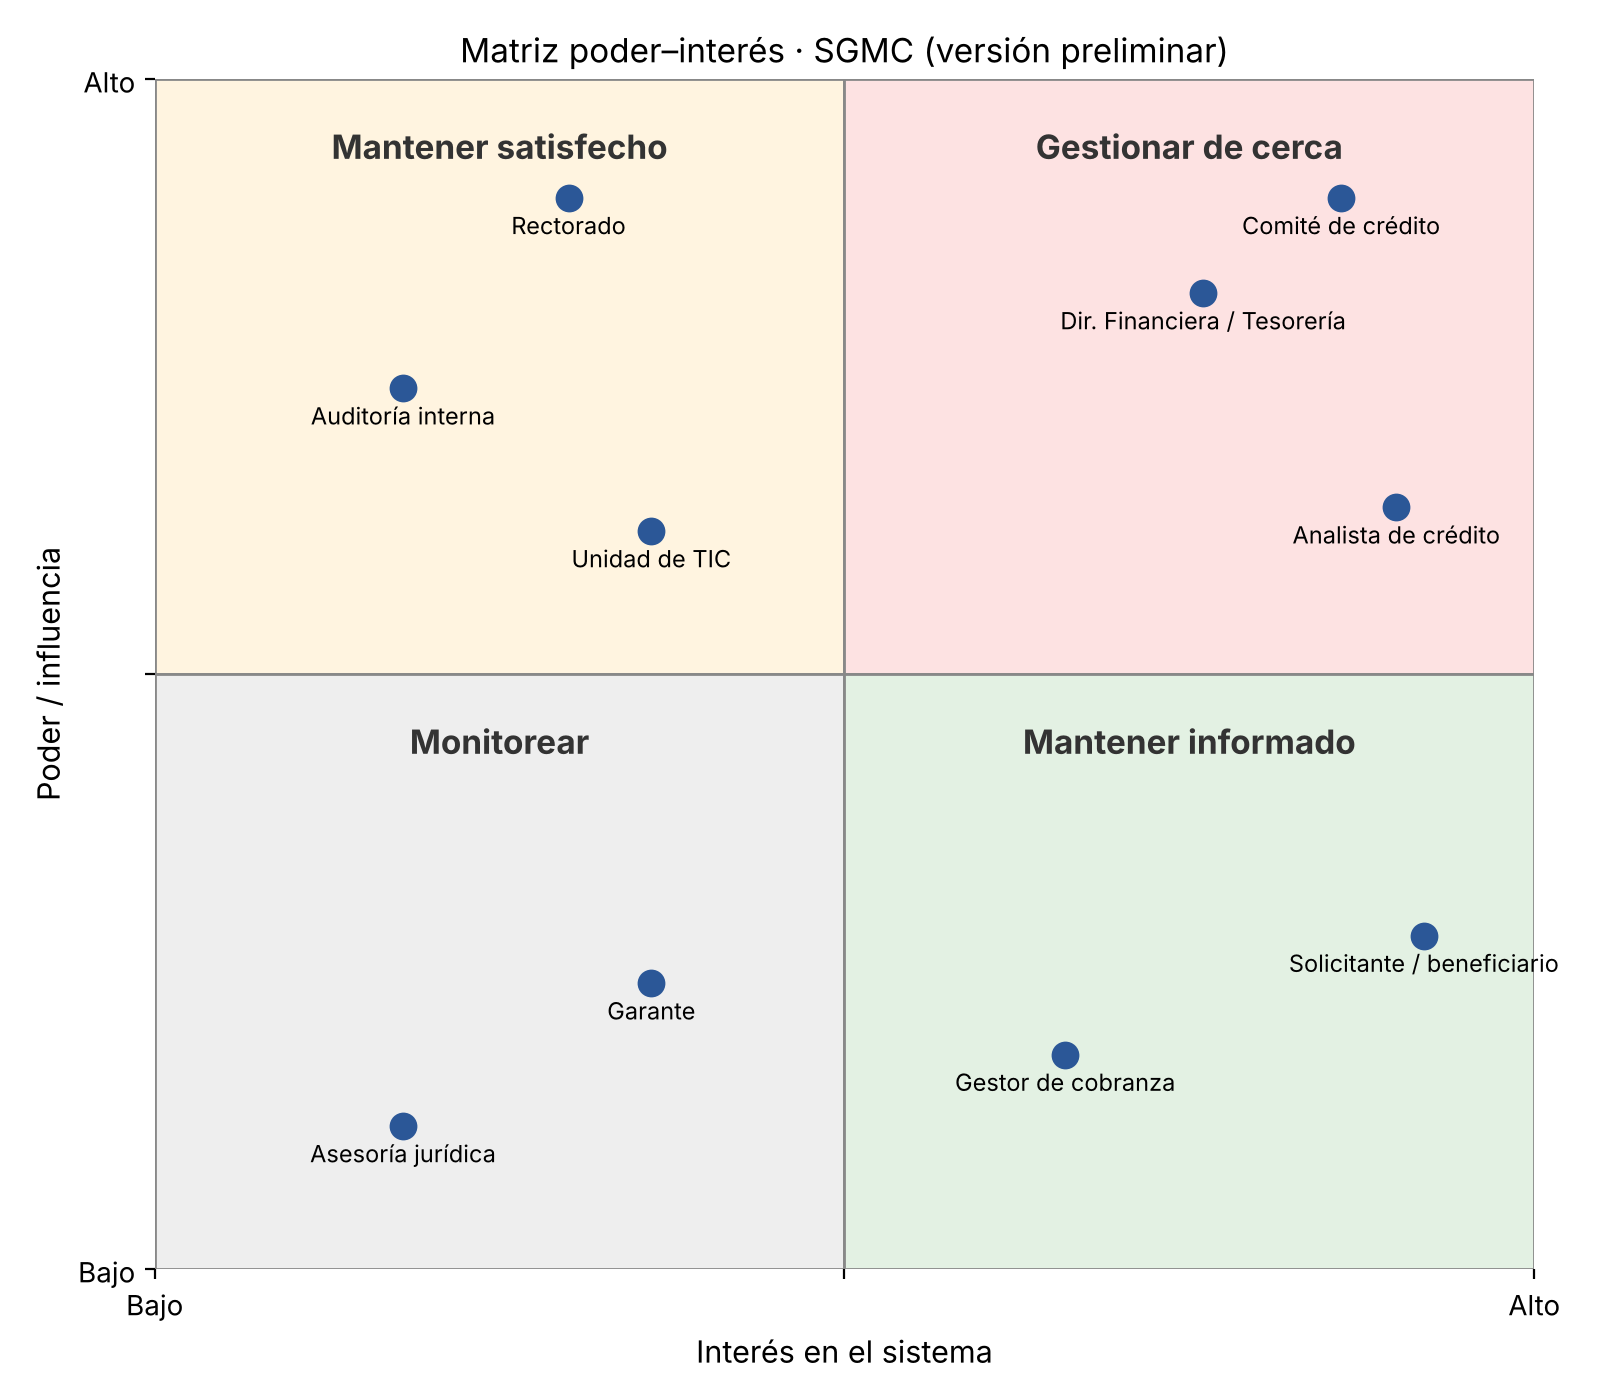
\includegraphics[width=0.75\textwidth]{figuras/matriz_poder_interes.png}
\caption{Matriz poder--interés de las partes interesadas del SGMC.}
\label{fig:matriz}
\end{figure}

\subsection{Estrategia de participación}

\begin{itemize}
\item \textbf{Gestionar de cerca} (comité, tesorería y analista): participan en entrevistas individuales y en la validación de los requisitos. El analista, por su alta disponibilidad, es la fuente principal para describir el proceso actual.
\item \textbf{Mantener satisfecho} (rectorado, auditoría y TIC): se les consulta en momentos puntuales, en especial sobre restricciones normativas, de control y técnicas, y se les envía un resumen de avance.
\item \textbf{Mantener informado} (solicitantes y gestor de cobranza): por ser muchos o tener poco poder de decisión, se recoge su opinión mediante el cuestionario y se les comunican los cambios que los afectan.
\item \textbf{Monitorear} (garante y asesoría jurídica): se revisa su situación al cerrar cada etapa; asesoría jurídica se consulta solo si surgen dudas sobre contratos o garantías.
\end{itemize}

El analista de crédito y el comité tienen la mayor carga de conocimiento del proceso, pero el comité tiene baja disponibilidad. Este conflicto es un riesgo para la elicitación: si el comité no puede asistir, se pedirá que delegue en un miembro y que las decisiones se validen después por escrito.

